\documentclass[mastertmp.tex]{subfiles}
\begin{document}
% Create a dedicated folder for the Figures
%\exec{[ ! -d ../Figures ] && mkdir ../Figures}

 Normal \LaTeX equation (it will look nice, but not always make sense)
\begin{equation} \label{eq:GeneralVolumeIntegral}
	V=\int {\int {f\left(x , y , z\right)}{\;z}}{\;dj\left(p , y
	\right)}
\end{equation}

Equations with numbering
% example to use maxima notation:
\begin{subequations} \label{ChgEllipCoord}
	\begin{align}
		\maxieq{r^2 = (x/a)^2 + (y/b)^2} \\
		\maxieq{x = a*r*cos(\theta)} \label{ChgEllipCoord1}\\
		\maxieq{y = b*r*sin(\theta)} \label{ChgEllipCoord2}
	\end{align}
\end{subequations}

This is a derivative with maxima code: $\displaystyle \maxieq{diff(f(x),x)}$

% Example gnuplot code (finish every line with semicolon):
\begin{figure}[htb!]
	\gnuplot{Caption}{test}{
		set xlabel "$x$";
		splot tan(x), sin(x);
	}{scale=0.8}
\end{figure}
The figure depicted in \Cref{fig:test} is made with Gnuplot


%% Uncomment and change path to code to test loading from file:
%\begin{figure}[htb!]
%	\gnuplotfile{Caption
%	}{LabelAndFileName}{path/file.gp}
%\end{figure}

\begin{figure}[htb!]
	\centering
	\gnuplotcmd{FileGnuplot}{
		% Example from the documentation demo_4.4/contours.1.gnu
		set samples 20, 20;
		set isosamples 21, 21;
		set contour base;
		set title "3D gnuplot demo - contour plot";
		set xlabel "X axis";
		set ylabel "Y axis";
		set zlabel "Z axis";
		set zlabel  offset character 1, 0, 0 font "" textcolor lt -1 norotate;
		splot x*y;
	}
	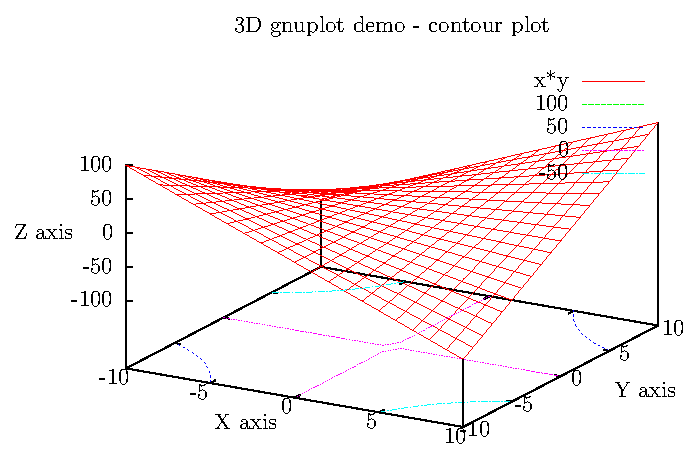
\includegraphics[]{Figures/FileGnuplot.eps}
	\caption{My Caption \label{label}}
\end{figure}

\begin{maximacmd}
   plot2d([cos(x),sin(x^2)], [x,-3,3],
          [plot_format, gnuplot],
          [gnuplot_term, ps],
          [run_viewer,false],
          [gnuplot_out_file,"grafico1.eps"]);
\end{maximacmd}
% DON'T EVER FORGET THIS LINE:
\IfFileExists{grafico1.eps}{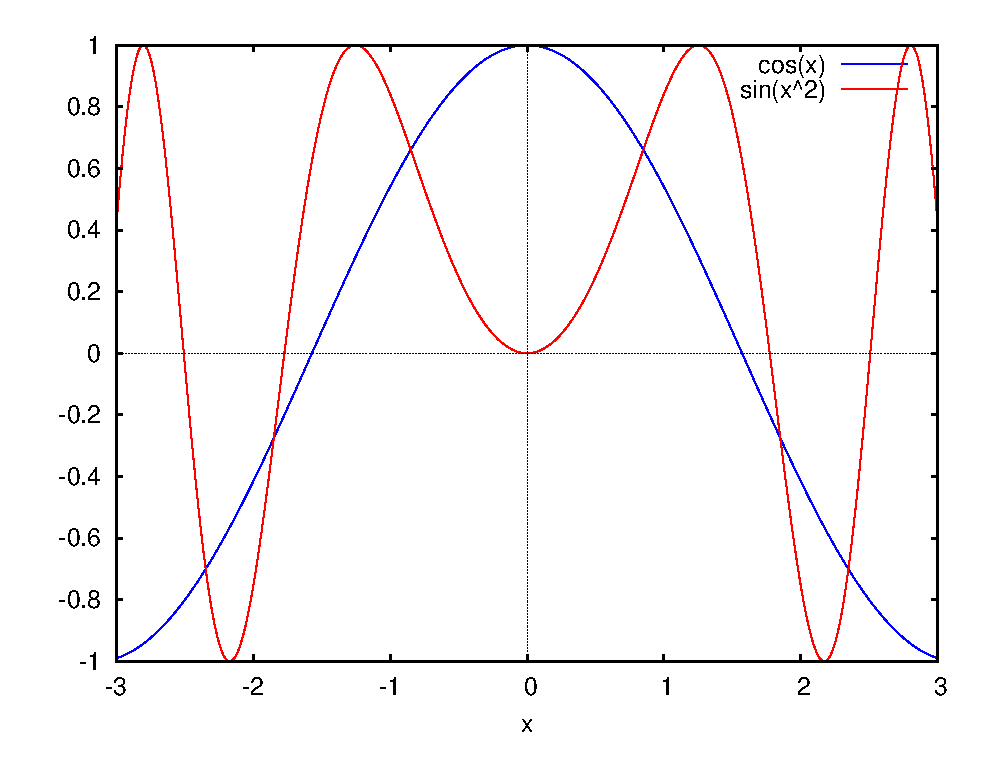
\includegraphics[scale=0.60]{grafico1.eps}}{}

\begin{maximaplot}{3d}{test2}{sin(x),[x,-4,4],[y,-4,4],
			[grid,50,50],[gnuplot_pm3d,true],
			[xlabel,"$\\Phi(x)$"],
			[gnuplot_preamble,"set pm3d at s;unset surface;set contour;
			set cntrparam levels 20; unset key; set border 0"]}
			{scale=0.8}
\end{maximaplot}

An equation goes here, and a 2D figure goes above

\[
 \begin{maxima}
 f:x/(x^3 - 3*x +2),
 tex('integrate(f,x)),
 print("="),
 tex(integrate(f,x)),
 print("+K")
 \end{maxima}
\]
\textbf{If you don't see anything above, run latex again} (you will always
need two runs for \textsc{maximacmd} and \textsc{maxima} commands, but
not for \textsc{maxieq}). The last figure

\end{document}
